%!TEX root = lecture_slides.tex
%%%%%%%%%%%%%%%%%%%%%%%%%%%%%%%%%%%%%%%%
%Some macros for the Venn Diagrams
\def\EventA{(-0.35,0) circle (1.2)}
\def\EventB{(1.35,0) circle (1.2)}
\def\EventC{(-0.35,0) circle (0.6)}
\def\EventD{(0,0) circle (1.6)}
\def\SampleSpace{(-2,-2) rectangle (3,2)}
%%%%%%%%%%%%%%%%%%%%%%%%%%%%%%%%%%%%%%%%
\section{Bayes' Rule and the Base Rate Fallacy}
%%%%%%%%%%%%%%%%%%%%%%%%%%%%%%%%%%%%%%%%

\begin{frame}
\centering \Huge Four Volunteers Please!

\end{frame}
%%%%%%%%%%%%%%%%%%%%%%%%%%%%%%%%%%%%%%%%
\begin{frame}
\frametitle{The Lie Detector Problem}
\begin{block}{From accounting records, we know that 10\% of employees in the store are stealing merchandise.}\end{block}
\begin{block}{The managers want to fire the thieves, but their only tool in distinguishing is a lie detector test that is 80\% accurate:}
	\begin{eqnarray*}
	\mbox{Innocent } &\Rightarrow& \mbox{Pass test with } 80\% \mbox{ Probability}\\
	\mbox{Thief } &\Rightarrow& \mbox{Fail test with } 80\% \mbox{ Probability}
	\end{eqnarray*}
\end{block}

\pause
\begin{alertblock}{What is the probability that someone is a thief \emph{given} that she has failed the lie detector test?\hfill
\includegraphics[scale = 0.03]{./images/clicker} }
\end{alertblock}

\end{frame}
%%%%%%%%%%%%%%%%%%%%%%%%%%%%%%%%%%%%%%%%

\begin{frame}
\frametitle{Monte Carlo Simulation -- Roll a 10-sided Die Twice}
Managers will split up and visit employees. Employees roll the die twice \alert{but keep the results secret!}
\vspace{1em}
\begin{block}{First Roll -- Thief or not?}
$0 \Rightarrow$ Thief, $1-9 \Rightarrow$ Innocent
\end{block}

\begin{block}{Second Roll -- Lie Detector Test}
$0,1 \Rightarrow$ Incorrect Test Result, $2-9$ Correct Test Result
\end{block}
\begin{table}
	\begin{tabular}{l|cc}
	&0 or 1&2--9\\
	\hline
	Thief&Pass&\alert{Fail}\\
	Innocent&\alert{Fail} &Pass
	\end{tabular}
\end{table}

\end{frame}
%%%%%%%%%%%%%%%%%%%%%%%%%%%%%%%%%%%%%%%%
\begin{frame}
\frametitle{What percentage of those who failed the test are guilty?}
\begin{block}{\# Who Failed Lie Detector Test:}

\end{block}


\begin{block}{\# Of Thieves Among Those Who Failed:}

\end{block}

\end{frame}
%%%%%%%%%%%%%%%%%%%%%%%%%%%%%%%%%%%%%%%%
\begin{frame}
\frametitle{Base Rate Fallacy -- Failure to Consider Prior Information}

\begin{block}{Base Rate -- Prior Information}
Before the test we know that 10\% of Employees are stealing.
\end{block}
\vspace{2em}
\begin{alertblock}{People tend to focus on the fact that the test is 80\% accurate and ignore the fact that only 10\% of the employees are theives. }
\end{alertblock}

\end{frame}
%%%%%%%%%%%%%%%%%%%%%%%%%%%%%%%%%%%%%%%%
\begin{frame}
\frametitle{Thief (Y/N), Lie Detector (P/F)}
\footnotesize
\begin{table}
\begin{tabular}{|c|cccccccccc|}
\hline
&0&1&2&3&4&5&6&7&8&9\\
\hline
0&\textcolor{blue}{YP}&\textcolor{blue}{YP}&\textcolor{red}{YF}&\textcolor{red}{YF}&\textcolor{red}{YF}&\textcolor{red}{YF}&\textcolor{red}{YF}&\textcolor{red}{YF}&\textcolor{red}{YF}&\textcolor{red}{YF}\\
1&\textcolor{red}{NF}&\textcolor{red}{NF}&\textcolor{blue}{NP}&\textcolor{blue}{NP}&\textcolor{blue}{NP}&\textcolor{blue}{NP}&\textcolor{blue}{NP}&\textcolor{blue}{NP}&\textcolor{blue}{NP}&\textcolor{blue}{NP}\\
2&\textcolor{red}{NF}&\textcolor{red}{NF}&\textcolor{blue}{NP}&\textcolor{blue}{NP}&\textcolor{blue}{NP}&\textcolor{blue}{NP}&\textcolor{blue}{NP}&\textcolor{blue}{NP}&\textcolor{blue}{NP}&\textcolor{blue}{NP}\\
3&\textcolor{red}{NF}&\textcolor{red}{NF}&\textcolor{blue}{NP}&\textcolor{blue}{NP}&\textcolor{blue}{NP}&\textcolor{blue}{NP}&\textcolor{blue}{NP}&\textcolor{blue}{NP}&\textcolor{blue}{NP}&\textcolor{blue}{NP}\\
4&\textcolor{red}{NF}&\textcolor{red}{NF}&\textcolor{blue}{NP}&\textcolor{blue}{NP}&\textcolor{blue}{NP}&\textcolor{blue}{NP}&\textcolor{blue}{NP}&\textcolor{blue}{NP}&\textcolor{blue}{NP}&\textcolor{blue}{NP}\\
5&\textcolor{red}{NF}&\textcolor{red}{NF}&\textcolor{blue}{NP}&\textcolor{blue}{NP}&\textcolor{blue}{NP}&\textcolor{blue}{NP}&\textcolor{blue}{NP}&\textcolor{blue}{NP}&\textcolor{blue}{NP}&\textcolor{blue}{NP}\\
6&\textcolor{red}{NF}&\textcolor{red}{NF}&\textcolor{blue}{NP}&\textcolor{blue}{NP}&\textcolor{blue}{NP}&\textcolor{blue}{NP}&\textcolor{blue}{NP}&\textcolor{blue}{NP}&\textcolor{blue}{NP}&\textcolor{blue}{NP}\\
7&\textcolor{red}{NF}&\textcolor{red}{NF}&\textcolor{blue}{NP}&\textcolor{blue}{NP}&\textcolor{blue}{NP}&\textcolor{blue}{NP}&\textcolor{blue}{NP}&\textcolor{blue}{NP}&\textcolor{blue}{NP}&\textcolor{blue}{NP}\\
8&\textcolor{red}{NF}&\textcolor{red}{NF}&\textcolor{blue}{NP}&\textcolor{blue}{NP}&\textcolor{blue}{NP}&\textcolor{blue}{NP}&\textcolor{blue}{NP}&\textcolor{blue}{NP}&\textcolor{blue}{NP}&\textcolor{blue}{NP}\\
9&\textcolor{red}{NF}&\textcolor{red}{NF}&\textcolor{blue}{NP}&\textcolor{blue}{NP}&\textcolor{blue}{NP}&\textcolor{blue}{NP}&\textcolor{blue}{NP}&\textcolor{blue}{NP}&\textcolor{blue}{NP}&\textcolor{blue}{NP}\\
\hline
\end{tabular}
\caption{Each outcome in the table is equally likely. The 26 given in red correspond to failing the test, but only 8 of these (YF) correspond to being a thief.}
\end{table}
\end{frame}
%%%%%%%%%%%%%%%%%%%%%%%%%%%%%%%%%%%%%%%%
\begin{frame}
\frametitle{Base Rate of Thievery is 10\%}

% Set the overall layout of the tree
\tikzstyle{level 1}=[level distance=3.5cm, sibling distance=3.5cm]
\tikzstyle{level 2}=[level distance=3.5cm, sibling distance=2.5cm]

% Define styles for bags and leafs
\tikzstyle{bag} = [text width=4em, text centered]
\tikzstyle{end} = [circle, minimum width=3pt,fill, inner sep=0pt]
\tikzstyle{tip} = [circle,fill, minimum height = 3pt, inner sep=0pt]
\begin{figure}
\centering
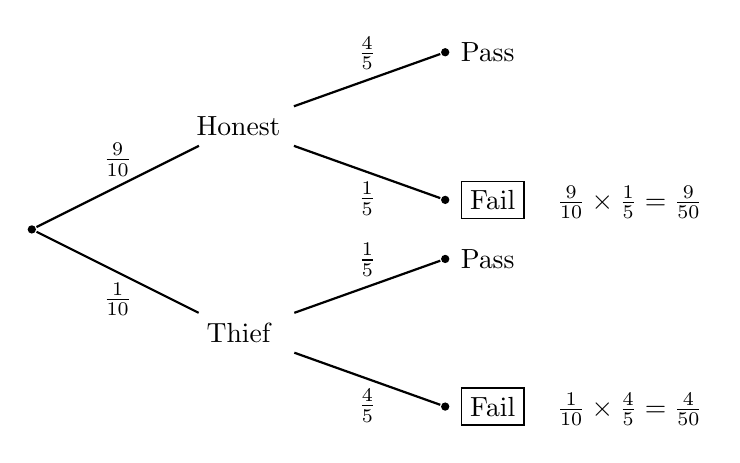
\begin{tikzpicture}[scale = 0.75,thick,grow=right]
\node[tip]{}
    child {
        node[bag] {Thief}        
        child {
                node[end, label=right:
                    {\alert{\fbox{Fail} $\;\;\; \frac{1}{10} \times \frac{4}{5} = \frac{4}{50}$}}] {}
                edge from parent
                node[below]  {$\frac{4}{5}$}
            }
            child {
                node[end, label=right:
                    {Pass}] {}
                edge from parent
                node[above] {$\frac{1}{5}$}
            }
            edge from parent 
            node[below]  {$\frac{1}{10}$}
    }
    child {
        node[bag] {Honest}        
        child {
                node[end, label=right:
                    {\alert{\fbox{Fail} $\;\;\; \frac{9}{10} \times \frac{1}{5} = \frac{9}{50}$}}] {}
                edge from parent
                node[below]  {$\frac{1}{5}$}
            }
            child {
                node[end, label=right:
                    {Pass}] {}
                edge from parent
                node[above] {$\frac{4}{5}$}
            }
        edge from parent         
            node[above] {$\frac{9}{10}$}
    };
\end{tikzpicture}
\caption{Although $\frac{9}{50} + \frac{4}{50} = \frac{13}{50}$ fail the test, only $\frac{4/50}{13/50} = \frac{4}{13} \approx 0.31$ are actually theives!}
\end{figure}


\end{frame}
%%%%%%%%%%%%%%%%%%%%%%%%%%%%%%%%%%%%%%%%
\begin{frame}
\frametitle{Deriving Bayes' Rule}
Intersection is symmetric: $A\cap B = B\cap A$ so $P(A\cap B) = P(B \cap A)$ \pause  By the definition of conditional probability,
	$$P(A|B) = \frac{P(A\cap B)}{P(B)}$$ \pause
And by the multiplication rule:
	$$P(B\cap A) = P(B|A)P(A)$$ \pause
Finally, combining these
	$$P(A|B) = \frac{P(B|A)P(A)}{P(B)}$$
\end{frame}
%%%%%%%%%%%%%%%%%%%%%%%%%%%%%%%%%%%%%%%%
\begin{frame}
\frametitle{Understanding Bayes' Rule}
$$\boxed{P(A|B) = \frac{P(B|A)P(A)}{P(B)}}$$

\begin{block}
	{Reversing the Conditioning}
	Express $P(A|B)$ in terms of $P(B|A)$. \emph{Relative magnitudes} of the two conditional probabilities determined by the ratio $P(A)/P(B)$.
\end{block}

\begin{block}
	{Base Rate}
	$P(A)$ is called the ``base rate'' or the ``prior probability.'' 
\end{block}

\begin{block}
	{Denominator}
	Typically, we calculate $P(B)$ using the law of toal probability
\end{block}


\end{frame}
%%%%%%%%%%%%%%%%%%%%%%%%%%%%%%%%%%%%%%%%
\begin{frame}
\frametitle{In General $P(A|B) \neq P(B|A)$ \hfill 
\includegraphics[scale = 0.05]{./images/clicker}} 
\begin{block}{Question}
Most college students are Democrats. Does it follow that most Democrats are college students?  \hfill  \alert{(A = YES, B = NO)}
\end{block}

\pause

\begin{block}{Answer}
There are many more Democracts than college students: 
$$P(\mbox{Dem}) > P(\mbox{Student})$$ 
so $P(\mbox{Student}|\mbox{Dem})$ is small even though $P(\mbox{Dem}|\mbox{Student})$ is large.
\end{block}
\end{frame}
%%%%%%%%%%%%%%%%%%%%%%%%%%%%%%%%%%%%%%%%
\begin{frame}
\frametitle{Solving the Lie Detector Problem with Bayes' Rule}
\footnotesize
\fbox{$T =$ Employee is a Thief, $F = $ Employee Fails Lie Detector Test}
\normalsize
\vspace{1em}
$$P(T|F) = \frac{P(F|T)P(T)}{P(F)}$$ \pause
\begin{eqnarray*}
	P(F) &=& P(F|T)P(T) + P(F|T^c)P(T^c)\\ \pause
		&=& 0.8 \times 0.1 + 0.2\times 0.9\\ \pause
		&=& \alert{0.08} + 0.18 = \alert{0.26} \pause
\end{eqnarray*}


$$P(T|F) = \frac{\alert{0.08}}{\alert{0.26}} = \pause \frac{8}{26} = \frac{4}{13} \approx 0.31$$
\end{frame}
%%%%%%%%%%%%%%%%%%%%%%%%%%%%%%%%%%%%%%%%
\begin{frame}
\singlespacing
\frametitle{``Odd'' Question \# 5}


There are two kinds of taxis: green cabs and blue cabs. Of all the cabs on the road, \alert{85\% are green cabs}. On a misty winter night a taxi sideswiped another car and drove off. \alert{A witness says it was a blue cab.} The witness is tested under conditions like those on the night of the accident, and \alert{80\% of the time she correctly reports the color of the cab that is seen}. That is, regardless of whether she is shown a blue or a green cab in misty evening light, she gets the color right 80\% of the time. 

\vspace{1em}
\begin{center}
\fbox{\begin{minipage}{0.85\textwidth}
\textcolor{blue}{Given that the witness said she saw a blue cab, what is the probability that a blue cab was the sideswiper?}
\end{minipage}}
\end{center}

\end{frame}

%%%%%%%%%%%%%%%%%%%%%%%%%%%%%%%%%%%%%%%%
\begin{frame}
\frametitle{Solving The Taxi Problem}
\footnotesize
\fbox{
\begin{minipage}{0.85\textwidth}
$G = $ Taxi is Green, $P(G) = 0.85$\\
$B = $ Taxi is Blue, $P(B) = 0.15$\\
$W_B = $ Witness says Taxi is Blue, $P(W_B|B) = 0.8, P(W_B|G) = 0.2$
\end{minipage}}
\normalsize

\vspace{1em}

\pause
$$P(B|W_B) = P(W_B|B)P(B)/P(W_B)$$
\pause
\begin{eqnarray*}
	P(W_B) &=& P(W_B|B) P(B) + P(W_B|G) P(G)\\ \pause
			&=& 0.8\times 0.15 + 0.2 \times 0.85 \\ \pause
			&=& \alert{0.12} + 0.17 = \alert{0.29}\\ \\ \pause
		P(B|W_B) &=& 0.12/0.29 = 12/29 \approx 0.41\\ \pause
		P(G|W_B) &=& 1 - (12/19) \approx 0.59 
	\end{eqnarray*}

\end{frame}

%%%%%%%%%%%%%%%%%%%%%%%%%%%%%%%%%%%%%%%%%
%\begin{frame}
%\frametitle{The Monty Hall Problem!}
%\begin{figure}
%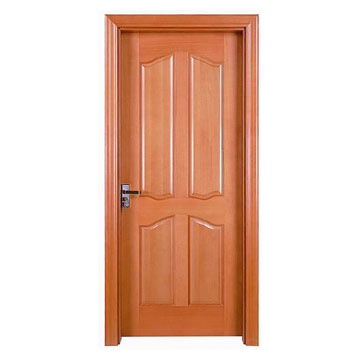
\includegraphics[scale = 0.28]{./images/door}
%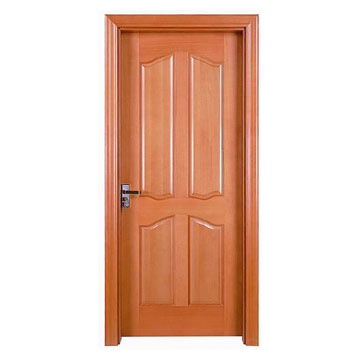
\includegraphics[scale = 0.28]{./images/door}
%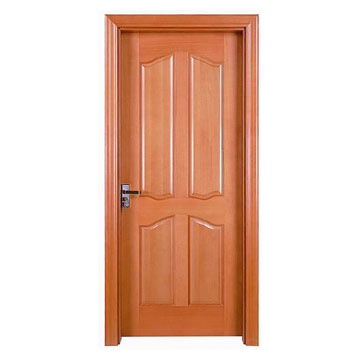
\includegraphics[scale = 0.28]{./images/door}
%\end{figure}
%\begin{figure}
%	\fbox{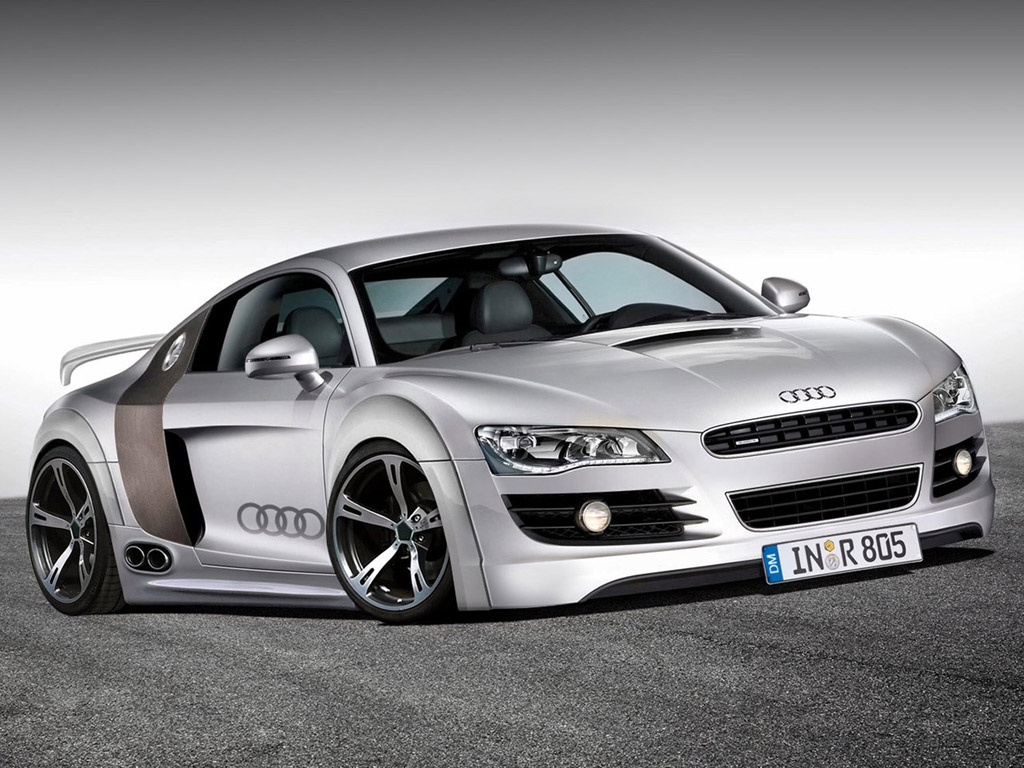
\includegraphics[scale = 0.08]{./images/car}}
%	\hspace{0.5em}
%	\fbox{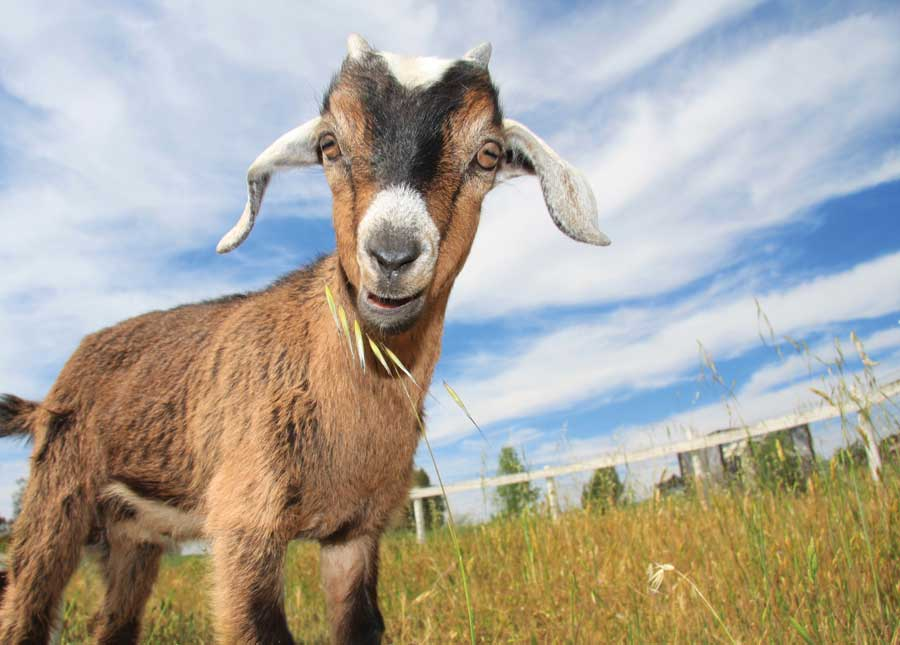
\includegraphics[scale = 0.095]{./images/goat}}
%	\hspace{0.5em}
%	\fbox{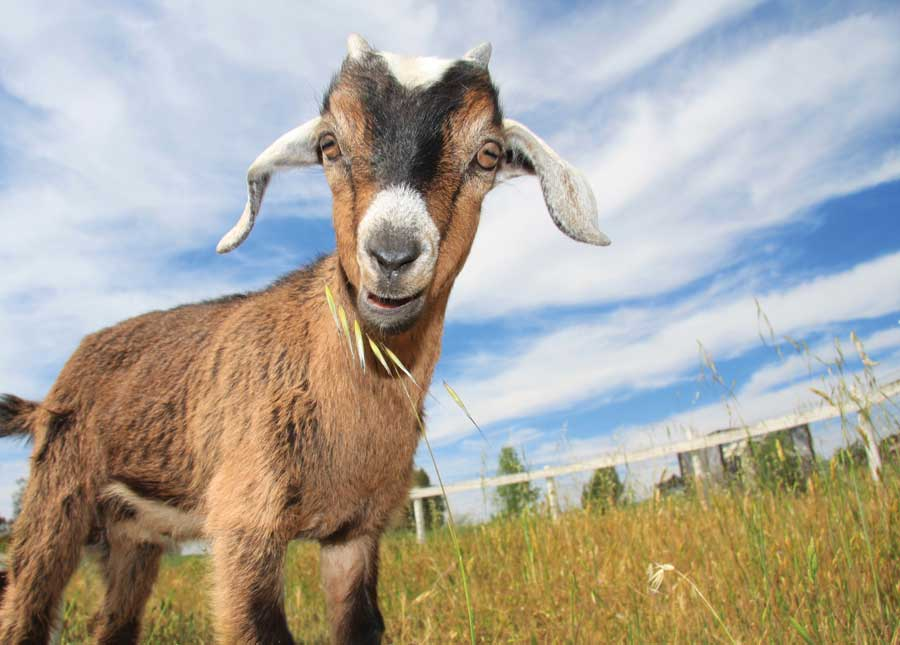
\includegraphics[scale = 0.095]{./images/goat}}
%\end{figure}
%\end{frame}
%%%%%%%%%%%%%%%%%%%%%%%%%%%%%%%%%%%%%%%%%
%
%
%\begin{frame}
%\frametitle{What is the probability that you win if you switch? \hfill 
\includegraphics[scale = 0.05]{./images/clicker}}
%\begin{figure}
%\centering
%	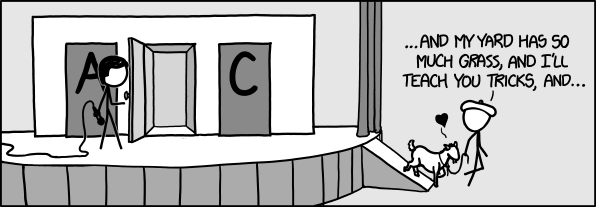
\includegraphics[scale = 0.55]{./images/monty_hall}
%\end{figure}
%\end{frame}
%
%%%%%%%%%%%%%%%%%%%%%%%%%%%%%%%%%%%%%%%%%%
%\begin{frame}
%
%\Huge Key Point -- Monte doesn't choose a door randomly: he \emph{always} shows you a goat.
%
%\end{frame}
%%%%%%%%%%%%%%%%%%%%%%%%%%%%%%%%%%%%%%%%%
%
%
%\begin{frame}
%\frametitle{Without loss of generality, suppose you chose door \#1}
%\begin{figure}[htbp]
%\begin{center}
%\small
%\synttree[Choose Door 1
%			[\emph{Car Behind Door 1}
%				[Switch	[\textbf{Lose}]	]	[Don't Switch	[\textbf{Win}]	]
%			]
%						[\emph{Car Behind Door 2}
%				[Switch	[\textbf{Win}]	]	[Don't Switch	[\textbf{Lose}]	]
%			]
%						[\emph{Car Behind Door 3}
%				[Switch	[\textbf{Win}]	]	[Don't Switch	[\textbf{Lose}]	]
%			]
%]
%\end{center}
%\end{figure}
%\end{frame}
%
%%%%%%%%%%%%%%%%%%%%%%%%%%%%%%%%%%%%%%%%%
\section{Overview of Random Variables}
%%%%%%%%%%%%%%%%%%%%%%%%%%%%%%%%%%%%%%%%%

\begin{frame}
  \begin{center}
  \Huge Random Variables
  \end{center}
\end{frame}
%%%%%%%%%%%%%%%%%%%%%%%%%%%%%%%%%%%%%%%%
%Some macros for diagrams of random variables
\def\RVraw{(-2.5,0) circle [radius=1.7]
	(-2.5,0) circle [radius=1.7]
	(2.5,0) circle [radius=1.7]
	node [above left] at (-3.75,1.25) {$S$}
	node [above right] at (3.75,1.25) {$\mathbb{R}$}
	%node [above] at (0,2) {$X\colon S \mapsto \mathbb{R}$}
}
%%%%%%%%%%%%%%%%%%%%%%%%%%%%%%%%%%%%%%%%
\begin{frame}
  \frametitle{Random Variables}
  \begin{quote}
    A random variable is neither random nor a variable.
  \end{quote}
\begin{block}{Random Variable (RV): $X$}
  A \emph{fixed} function that assigns a \emph{number} to each basic outcome of a random experiment.
\end{block}
 
\begin{block}{Realization: $x$}
A particular numeric value that an RV could take on. We write $\{X = x\}$ to refer to the \emph{event} that the RV $X$ took on the value $x$.  
\end{block}
 
\begin{block}{Support Set (aka Support)}
The set of all possible realizations of a RV.
\end{block}
 
\end{frame}
%%%%%%%%%%%%%%%%%%%%%%%%%%%%%%%%%%%%%%%%
\begin{frame}
  \frametitle{Random Variables (continued)}
\begin{block}{Notation}
Capital latin letters for RVs, e.g.\ $X,Y,Z$, and the corresponsing lowercase letters for their realizations, e.g.\ $x,y,z$.
\end{block}

\begin{block}{Intuition}
  You can think of an RV as a machine that spits out random numbers: although the machine is deterministic, its inputs, the outcomes of a random experiment, are not.
\end{block}
\end{frame}
%%%%%%%%%%%%%%%%%%%%%%%%%%%%%%%%%%%%%%%%%
\begin{frame}
\frametitle{Example: Coin Flip Random Variable}

\begin{figure}
\centering
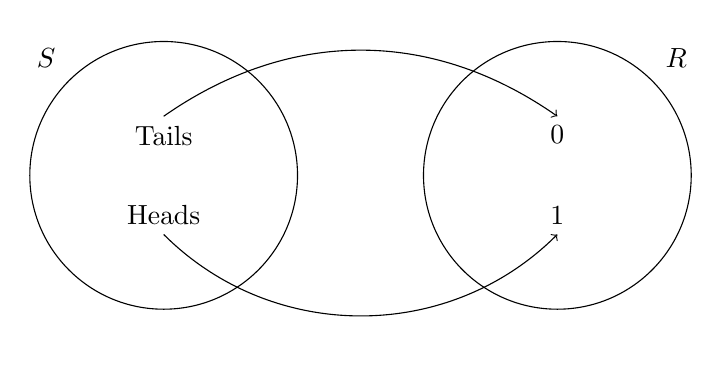
\begin{tikzpicture}
\draw \RVraw;
\draw [->] (-2.5,0.75) node [below]{Tails} to [out=35,in=145] (2.5,0.75) node [below]{$0$};
\draw [->] (-2.5,-0.75) node [above]{Heads} to [out=315,in=225] (2.5,-0.75) node [above]{$1$};
\end{tikzpicture}
\caption{This random variable assigns numeric values to the random experiment of flipping a fair coin once: Heads is assigned 1 and Tails 0.}
\end{figure}
\end{frame}
%%%%%%%%%%%%%%%%%%%%%%%%%%%%%%%%%%%%%%%%%%
\begin{frame}
  \frametitle{Which of these is a realization of the Coin Flip RV?\hfill
\includegraphics[scale = 0.05]{./images/clicker}}
  \begin{enumerate}[(a)]
    \item Tails
    \item 2
    \item 0 
    \item Heads
    \item 1/2
  \end{enumerate}
\end{frame}
%%%%%%%%%%%%%%%%%%%%%%%%%%%%%%%%%%%%%%%%%%
\begin{frame}
  \frametitle{What is the support set of the Coin Flip RV?\hfill
\includegraphics[scale = 0.05]{./images/clicker}}
  \begin{enumerate}[(a)]
    \item $\left\{ \mbox{Heads}, \mbox{Tails} \right\}$ 
    \item 1/2 
    \item 0 
    \item $\left\{ 0,1 \right\}$
    \item 1
  \end{enumerate}
\end{frame}
%%%%%%%%%%%%%%%%%%%%%%%%%%%%%%%%%%%%%%%%%%
\begin{frame}
  \frametitle{Let $X$ denote the Coin Flip RV \hfill
\includegraphics[scale = 0.05]{./images/clicker}}
  What is $P\left( X=1 \right)$?

  \vspace{1em}

  \begin{enumerate}[(a)]
    \item 0 
    \item 1  
    \item 1/2 
    \item Not enough information to determine
  \end{enumerate}
\end{frame}
%%%%%%%%%%%%%%%%%%%%%%%%%%%%%%%%%%%%%%%%%%
\begin{frame}
  \frametitle{Two Kinds of RVs: Discrete and Continuous}
  \begin{description}
    \item[Discrete] support set is discrete, e.g.\ $\left\{ 0,1,2 \right\}$,  $\left\{ \hdots, -2, -1, 0, 1, 2,\hdots \right\}$
    \item[Continuous] support set is continuous, e.g.\ $[-1,1]$, $\mathbb{R}$.
  \end{description}

  \vspace{1em}

  \alert{Start with the discrete case since it's easier, but most of the ideas we learn will carry over to the continuous case.}
\end{frame}
%%%%%%%%%%%%%%%%%%%%%%%%%%%%%%%%%%%%%%%%%%
\section{Probability Mass Functions}
%%%%%%%%%%%%%%%%%%%%%%%%%%%%%%%%%%%%%%%%%%
\begin{frame}

\centering \Huge Discrete Random Variables I

\end{frame}
%%%%%%%%%%%%%%%%%%%%%%%%%%%%%%%%%%%%%%%%
\begin{frame}
\frametitle{Probability Mass Function (pmf)}
 A function that gives $P(X=x)$ for any realization $x$ in the support set of a discrete RV $X$. We use the following notation for the pmf:
 $$p(x) = P(X =x)$$

 

\begin{alertblock}{Plug in a realization $x$, get out a probability  $p(x)$.}\end{alertblock}

 


\end{frame}
%%%%%%%%%%%%%%%%%%%%%%%%%%%%%%%%%%%%%%%%
\begin{frame}
\frametitle{Probability Mass Function for Coin Flip RV}

\begin{columns}
\column{0.25\textwidth}
$$X = \left\{ \begin{array}{l}  0, \mbox{Tails}\\ 1, \mbox{Heads}\end{array} \right.$$

\begin{eqnarray*}
	p(0) &=& 1/2\\
	p(1) &=& 1/2
\end{eqnarray*}


\column{0.75\textwidth}
\begin{figure}
\centering
\begin{tikzpicture}[scale = 1.5]
\draw [<->] (0,2) node [above]{$p(x)$} -- (0,0) -- (3,0) node [right]{$x$};
\draw [blue, thick] (0.75,0) node [black, below]{0} -- (0.75,1.5);
\draw [blue, thick] (2.25,0) node [black, below]{1} -- (2.25,1.5);
\draw [dashed, gray] (0, 1.5) node [black, left]{$1/2$} -- (3,1.5);
\draw [fill=blue] (2.25,1.51) circle [radius = 0.05];
\draw [fill=blue] (0.75,1.51) circle [radius = 0.05];
\end{tikzpicture}
\caption{Plot of pmf for Coin Flip Random Variable}
\end{figure}
\end{columns}


\end{frame}
%%%%%%%%%%%%%%%%%%%%%%%%%%%%%%%%%%%%%%%%


\begin{frame}
\frametitle{Important Note about Support Sets}
Whenever you write down the pmf of a RV, it is \alert{crucial} to also write down its Support Set. Recall that this is the set of \alert{\emph{all possible realizations for a RV}}. Outside of the support set, all probabilities are zero. In other words, the pmf is \alert{only defined} on the support.

\end{frame}
%%%%%%%%%%%%%%%%%%%%%%%%%%%%%%%%%%%%%%%%
\begin{frame}
\frametitle{Properties of Probability Mass Functions}

If $p(x)$ is the pmf of a random variable $X$, then
\begin{enumerate}[(i)]
	\item $0\leq p(x) \leq 1$ for all $x$ \vspace{1em}
	\item $\displaystyle \sum_{\mbox{all } x} p(x) = 1$
\end{enumerate}

\vspace{0.75em}
where ``all $x$'' is shorthand for ``all $x$ in the support of $X$.''
\end{frame}
%%%%%%%%%%%%%%%%%%%%%%%%%%%%%%%%%%%%%%%%


